% =====================================================================
%  ParadePaard - Employee Lifecycle Flow
%  Derived from the actual codebase:
%    Program/frontend/src/pages/*        (React page components)
%    Program/frontend/src/services/*     (API service DTOs)
%    Program/frontend/src/utils/permissionPolicy.ts
%    Program/microservice/*-service/src  (Java services & enums)
%
%  Compile with: pdflatex -> pdflatex  (two passes for cross-references)
% =====================================================================
\documentclass[11pt,a4paper]{article}

\usepackage[utf8]{inputenc}
\usepackage[T1]{fontenc}
\usepackage[a4paper,margin=2.2cm,headheight=15pt]{geometry}
\usepackage{xcolor}
\usepackage{booktabs}
\usepackage{tabularx}
\usepackage{array}
\usepackage{fancyhdr}
\usepackage{pdflscape}
\usepackage{enumitem}
\usepackage{tikz}
\usetikzlibrary{shapes.geometric, arrows.meta, positioning, calc, fit, backgrounds}
\usepackage[colorlinks=true, linkcolor=ppblue, urlcolor=ppblue, citecolor=ppblue]{hyperref}

% ---------------------------------------------------------------------
%  Colour palette
% ---------------------------------------------------------------------
\definecolor{ppblue}{RGB}{37,99,175}      % process steps
\definecolor{ppbluefill}{RGB}{223,235,250}
\definecolor{pporange}{RGB}{200,120,20}   % decisions
\definecolor{pporangefill}{RGB}{253,237,213}
\definecolor{ppgreen}{RGB}{34,139,87}     % automated emails
\definecolor{ppgreenfill}{RGB}{223,245,233}
\definecolor{ppred}{RGB}{183,46,46}       % rejection paths
\definecolor{ppredfill}{RGB}{250,226,226}
\definecolor{ppgrey}{RGB}{90,96,104}      % start / end terminals
\definecolor{ppgreyfill}{RGB}{231,233,236}
\definecolor{pphead}{RGB}{52,60,72}

% ---------------------------------------------------------------------
%  Helper: print code-like tokens with underscores safely
% ---------------------------------------------------------------------
\newcommand{\code}[1]{\texttt{\detokenize{#1}}}
\newcommand{\stage}[1]{\textbf{#1}}

% ---------------------------------------------------------------------
%  Headers and footers
% ---------------------------------------------------------------------
\pagestyle{fancy}
\fancyhf{}
\renewcommand{\headrulewidth}{0.4pt}
\renewcommand{\footrulewidth}{0.4pt}
\lhead{\textcolor{pphead}{\small ParadePaard}}
\rhead{\textcolor{pphead}{\small Employee Lifecycle Flow}}
\lfoot{\small Internal documentation \textemdash{} derived from source}
\rfoot{\small Page \thepage}

% ---------------------------------------------------------------------
%  TikZ node styles
% ---------------------------------------------------------------------
\tikzset{
  process/.style   = {rectangle, rounded corners=3pt, draw=ppblue, line width=0.9pt,
                      fill=ppbluefill, text=pphead, align=center,
                      minimum width=30mm, minimum height=11mm, font=\sffamily\small,
                      inner sep=3pt},
  decision/.style  = {diamond, draw=pporange, line width=0.9pt, fill=pporangefill,
                      text=pphead, align=center, aspect=1.7,
                      inner sep=1pt, font=\sffamily\footnotesize},
  email/.style     = {rectangle, draw=ppgreen, line width=0.9pt, dashed,
                      fill=ppgreenfill, text=pphead, align=center,
                      minimum width=28mm, minimum height=10mm, font=\sffamily\footnotesize,
                      inner sep=3pt},
  reject/.style    = {rectangle, rounded corners=1pt, draw=ppred, line width=0.9pt,
                      fill=ppredfill, text=pphead, align=center,
                      minimum width=27mm, minimum height=10mm, font=\sffamily\footnotesize,
                      inner sep=3pt},
  terminal/.style  = {rectangle, rounded corners=10pt, draw=ppgrey, line width=1pt,
                      fill=ppgreyfill, text=pphead, align=center,
                      minimum width=30mm, minimum height=11mm, font=\sffamily\small\bfseries,
                      inner sep=3pt},
  flow/.style      = {-{Stealth[length=2.4mm]}, line width=0.8pt, draw=pphead},
  flowlab/.style   = {font=\sffamily\scriptsize, text=pphead, fill=white, inner sep=1.2pt},
  rejflow/.style   = {-{Stealth[length=2.4mm]}, line width=0.8pt, draw=ppred},
  mailflow/.style  = {-{Stealth[length=2.4mm]}, line width=0.7pt, draw=ppgreen, dashed},
}

% =====================================================================
\begin{document}

% ---------------------------------------------------------------------
%  TITLE PAGE
% ---------------------------------------------------------------------
\begin{titlepage}
\centering
\vspace*{2.2cm}
{\Huge\bfseries\textcolor{ppblue}{ParadePaard}\par}
\vspace{0.4cm}
{\LARGE The Complete Employee Lifecycle Flow\par}
\vspace{0.3cm}
{\large From public application to released payslip\par}
\vspace{1.4cm}

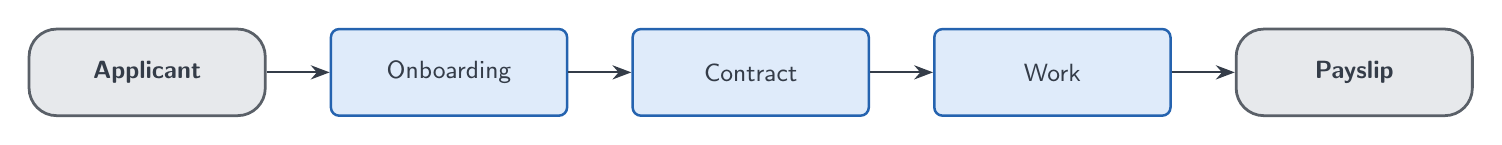
\begin{tikzpicture}
  \node[terminal] (a) {Applicant};
  \node[process, right=8mm of a] (b) {Onboarding};
  \node[process, right=8mm of b] (c) {Contract};
  \node[process, right=8mm of c] (d) {Work};
  \node[terminal, right=8mm of d] (e) {Payslip};
  \draw[flow] (a)--(b); \draw[flow] (b)--(c); \draw[flow] (c)--(d); \draw[flow] (d)--(e);
\end{tikzpicture}

\vspace{1.6cm}
{\large\bfseries Internal Process \& Permissions Reference\par}
\vspace{0.6cm}
\begin{minipage}{0.8\textwidth}
\centering\small
This document describes every stage an individual passes through in the
ParadePaard platform \textemdash{} covering \emph{both} the employee-facing journey and
the employer/administrator side of every step: which fields are captured,
which actions each role can take, which statuses exist, which automated
emails fire, and how permissions gate the whole flow. All content is derived
from the application source code, not invented.
\end{minipage}

\vfill
{\small Generated \today{} \quad\textbullet\quad ParadePaard HR / Payroll Platform\par}
\end{titlepage}

% ---------------------------------------------------------------------
%  TABLE OF CONTENTS
% ---------------------------------------------------------------------
\tableofcontents
\thispagestyle{fancy}
\clearpage

% ---------------------------------------------------------------------
%  LEGEND
% ---------------------------------------------------------------------
\section*{How to read the flowchart}
\addcontentsline{toc}{section}{How to read the flowchart}

The lifecycle is drawn as \emph{two} separate flows on the following pages.
\textbf{Flow~1 \textemdash{} Hiring \& Onboarding} runs from first contact up to the
moment the employee can see their finalised contract, where it ends.
\textbf{Flow~2 \textemdash{} Work \& Payroll} is a fresh flow that starts once the
employee is active: it begins at shift planning and runs through to a received
payslip. Every box carries the section number (\S) of the page that explains it
in detail. Box shapes and colours encode the kind of step:

\vspace{0.4em}
\begin{center}
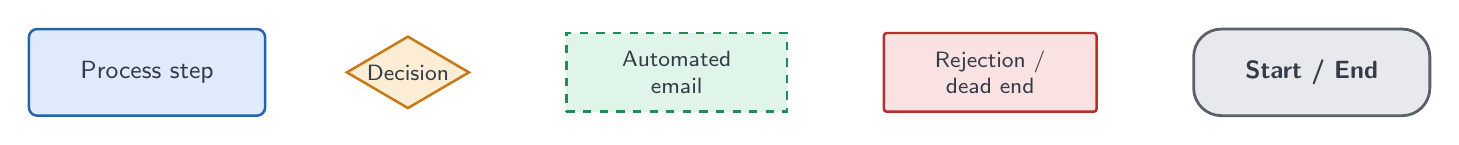
\begin{tikzpicture}[node distance=4mm]
  \node[process]  (p) {Process step};
  \node[decision, right=10mm of p] (d) {Decision};
  \node[email, right=12mm of d] (m) {Automated\\email};
  \node[reject, right=12mm of m] (r) {Rejection /\\dead end};
  \node[terminal, right=12mm of r] (t) {Start / End};
\end{tikzpicture}
\end{center}

\vspace{0.4em}
\noindent\textbf{Two entry points.} A person can enter the system either as a
\emph{public applicant} who fills in the application form (\S\ref{sec:application}),
or be created directly by an administrator through \emph{admin onboarding}
(\S\ref{sec:onboarding}), which skips the application/review stages and
provisions an account, a contract draft and a temporary password in one step.

\clearpage

% =====================================================================
%  FLOW 1 - HIRING & ONBOARDING (landscape, ends at contract view)
% =====================================================================
\begin{landscape}
\thispagestyle{fancy}
\begin{center}
{\LARGE\bfseries Flow 1 \textemdash{} Hiring \& Onboarding}\\[1mm]
{\normalsize From first contact to a finalised, viewable contract \textemdash{} where this flow ends.}\\[3mm]
\end{center}

\noindent\makebox[\linewidth][c]{%
\resizebox{\linewidth}{!}{%
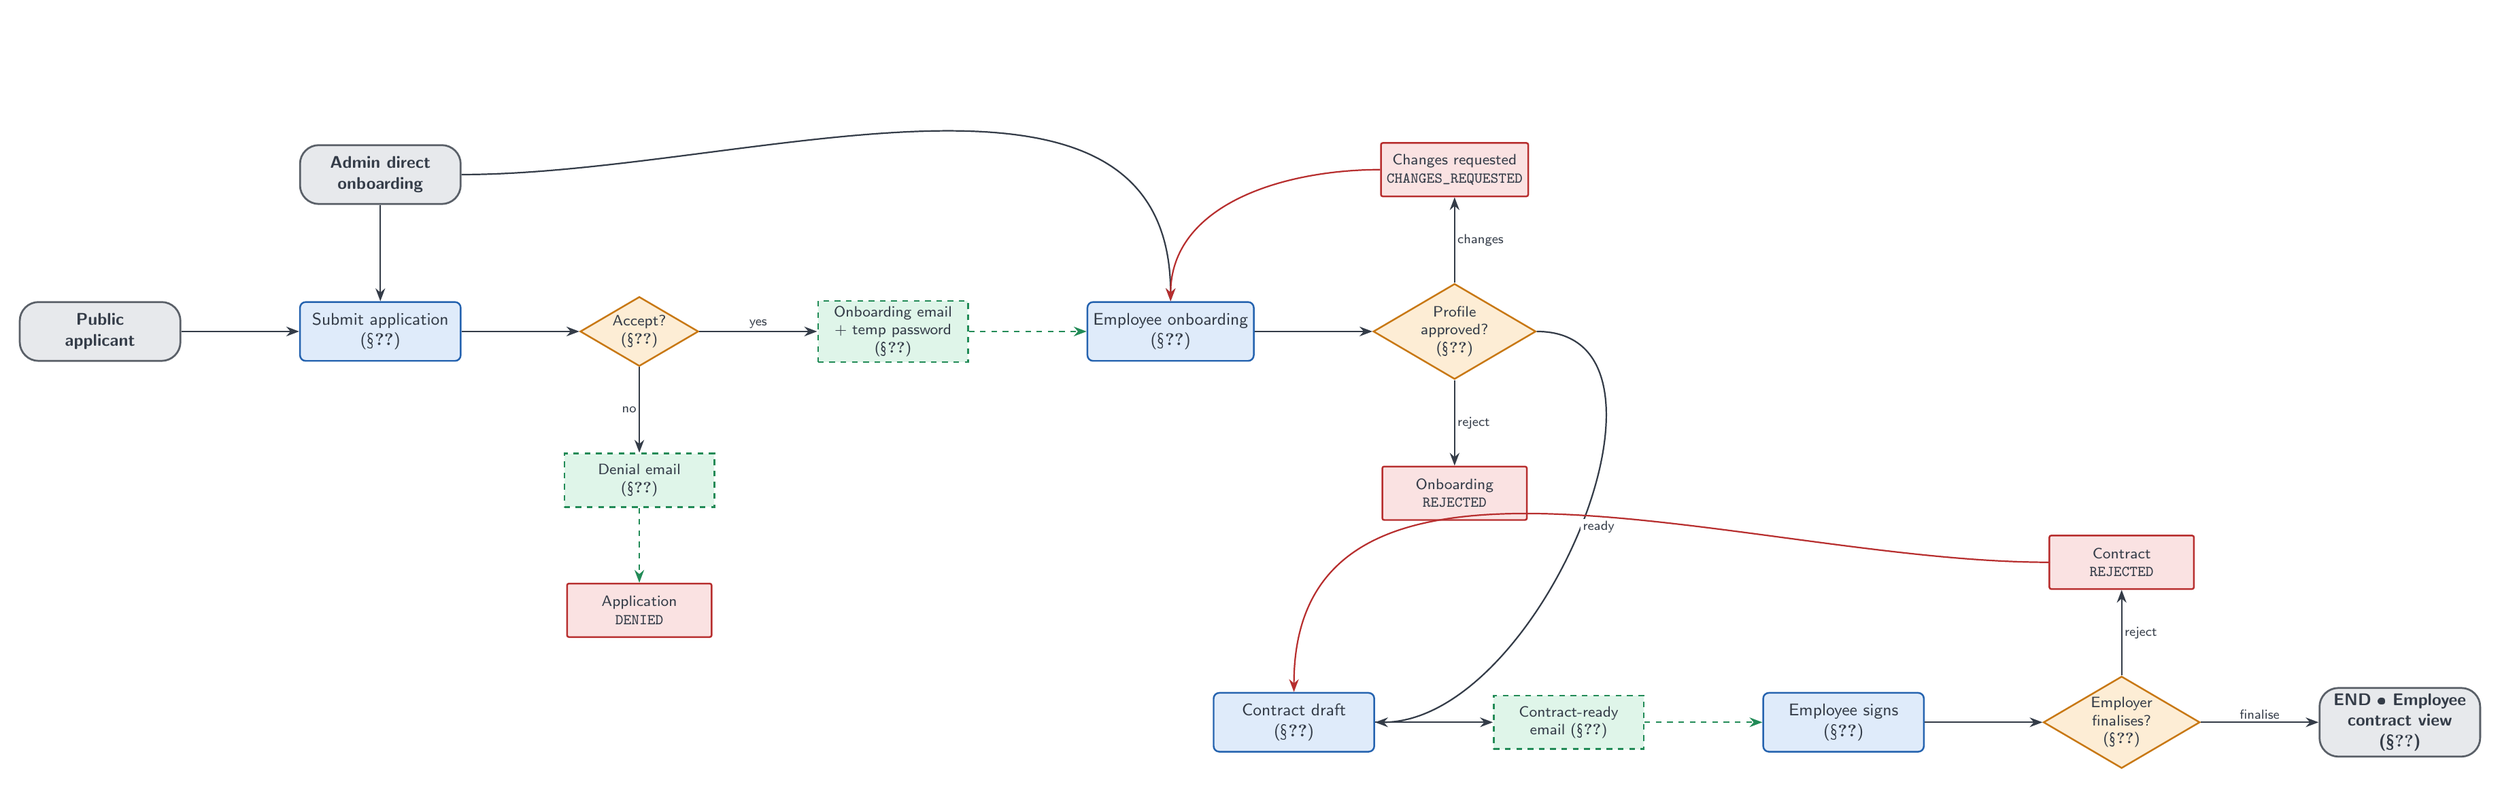
\begin{tikzpicture}[node distance=14mm and 22mm]

% ---------- Entry points ----------
\node[terminal] (start) {Public\\applicant};
\node[process, right=of start] (apply) {Submit application\\(\S\ref{sec:application})};
\node[decision, right=of apply] (accept) {Accept?\\(\S\ref{sec:appreview})};

% admin alternate entry (above)
\node[terminal, above=18mm of apply] (adminstart) {Admin direct\\onboarding};

% deny branch (below accept)
\node[email,  below=16mm of accept] (denymail) {Denial email\\(\S\ref{sec:emails})};
\node[reject, below=14mm of denymail] (denied) {Application\\\code{DENIED}};

% accept -> account + onboarding email
\node[email, right=of accept] (acctmail) {Onboarding email\\+ temp password\\(\S\ref{sec:emails})};
\node[process, right=of acctmail] (onboard) {Employee onboarding\\(\S\ref{sec:onboarding})};
\node[decision, right=of onboard] (profok) {Profile\\approved?\\(\S\ref{sec:onbreview})};

% profile review branches
\node[reject, above=16mm of profok] (changes) {Changes requested\\\code{CHANGES_REQUESTED}};
\node[reject, below=16mm of profok] (onbreject) {Onboarding\\\code{REJECTED}};

% contract spine (second row, going right)
\node[process, below=32mm of onbreject, xshift=-30mm] (contract) {Contract draft\\(\S\ref{sec:contract})};
\node[email, right=of contract] (cmail) {Contract-ready\\email (\S\ref{sec:emails})};
\node[process, right=of cmail] (sign) {Employee signs\\(\S\ref{sec:signing})};
\node[decision, right=of sign] (finalize) {Employer\\finalises?\\(\S\ref{sec:contract})};
\node[reject, above=16mm of finalize] (creject) {Contract\\\code{REJECTED}};
\node[terminal, right=of finalize] (cview) {END \textbullet{} Employee\\contract view\\(\S\ref{sec:contractview})};

% ---------- Edges: application ----------
\draw[flow] (start) -- (apply);
\draw[flow] (apply) -- (accept);
\draw[flow] (accept) -- node[flowlab,left]{no} (denymail);
\draw[mailflow] (denymail) -- (denied);
\draw[flow] (accept) -- node[flowlab,above]{yes} (acctmail);
\draw[mailflow] (acctmail) -- (onboard);
\draw[flow] (adminstart) -- (apply);
\draw[flow] (adminstart.east) to[out=0,in=90] (onboard.north);

% ---------- Edges: onboarding ----------
\draw[flow] (onboard) -- (profok);
\draw[flow] (profok) -- node[flowlab,right]{changes} (changes);
\draw[rejflow] (changes.west) to[out=180,in=90] (onboard.north);
\draw[flow] (profok) -- node[flowlab,right]{reject} (onbreject);
\draw[flow] (profok.east) to[out=0,in=0] node[flowlab,right]{ready} (contract.east);

% ---------- Edges: contract ----------
\draw[flow] (contract) -- (cmail);
\draw[mailflow] (cmail) -- (sign);
\draw[flow] (sign) -- (finalize);
\draw[flow] (finalize) -- node[flowlab,right]{reject} (creject);
\draw[rejflow] (creject.west) to[out=180,in=90] (contract.north);
\draw[flow] (finalize) -- node[flowlab,above]{finalise} (cview);

\end{tikzpicture}%
}}

\end{landscape}
\clearpage

% =====================================================================
%  FLOW 2 - WORK & PAYROLL (landscape, fresh start at shift planning)
% =====================================================================
\begin{landscape}
\thispagestyle{fancy}
\begin{center}
{\LARGE\bfseries Flow 2 \textemdash{} Work \& Payroll}\\[1mm]
{\normalsize A new flow for an active employee \textemdash{} starts at shift planning and ends at a received payslip.}\\[3mm]
\end{center}

\noindent\makebox[\linewidth][c]{%
\resizebox{\linewidth}{!}{%
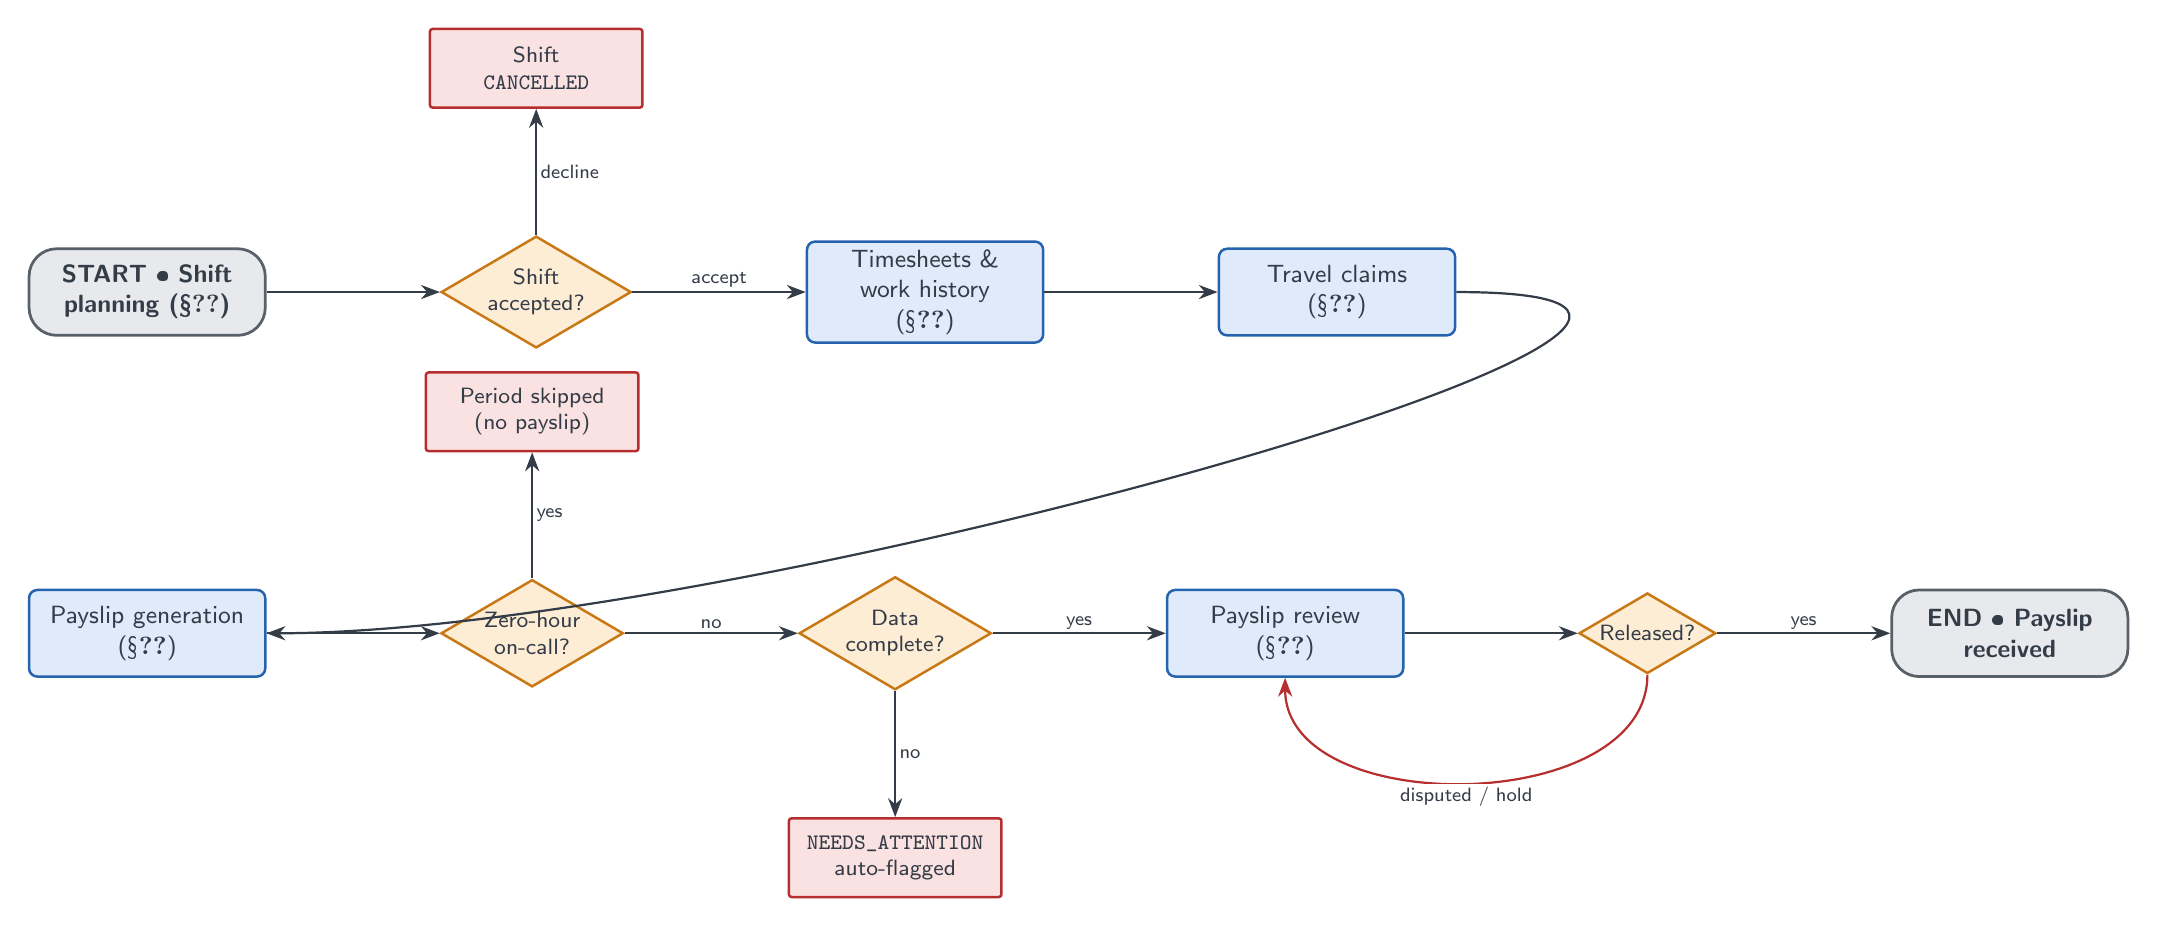
\begin{tikzpicture}[node distance=14mm and 22mm]

% ---------- Work row ----------
\node[terminal] (planning) {START \textbullet{} Shift\\planning (\S\ref{sec:planning})};
\node[decision, right=of planning] (shiftok) {Shift\\accepted?};
\node[reject, above=16mm of shiftok] (declined) {Shift\\\code{CANCELLED}};
\node[process, right=of shiftok] (timesheet) {Timesheets \&\\work history\\(\S\ref{sec:timesheets})};
\node[process, right=of timesheet] (travel) {Travel claims\\(\S\ref{sec:travel})};

% ---------- Payroll row ----------
\node[process, below=32mm of planning] (paygen) {Payslip generation\\(\S\ref{sec:payslipgen})};
\node[decision, right=of paygen] (zero) {Zero-hour\\on-call?};
\node[reject, above=16mm of zero] (skip) {Period skipped\\(no payslip)};
\node[decision, right=of zero] (datok) {Data\\complete?};
\node[reject, below=16mm of datok] (attention) {\code{NEEDS_ATTENTION}\\auto-flagged};
\node[process, right=of datok] (payreview) {Payslip review\\(\S\ref{sec:payslipreview})};
\node[decision, right=of payreview] (release) {Released?};
\node[terminal, right=of release] (gotpay) {END \textbullet{} Payslip\\received};

% ---------- Edges: work ----------
\draw[flow] (planning) -- (shiftok);
\draw[flow] (shiftok) -- node[flowlab,right]{decline} (declined);
\draw[flow] (shiftok) -- node[flowlab,above]{accept} (timesheet);
\draw[flow] (timesheet) -- (travel);
\draw[flow] (travel.east) to[out=0,in=0] (paygen.east);

% ---------- Edges: payroll ----------
\draw[flow] (paygen) -- (zero);
\draw[flow] (zero) -- node[flowlab,right]{yes} (skip);
\draw[flow] (zero) -- node[flowlab,above]{no} (datok);
\draw[flow] (datok) -- node[flowlab,right]{no} (attention);
\draw[flow] (datok) -- node[flowlab,above]{yes} (payreview);
\draw[flow] (payreview) -- (release);
\draw[flow] (release) -- node[flowlab,above]{yes} (gotpay);
\draw[rejflow] (release.south) to[out=-90,in=-90] node[flowlab,below]{disputed / hold} (payreview.south);

\end{tikzpicture}%
}}

\end{landscape}
\clearpage
% =====================================================================
%  STAGE 1 - APPLICATION
% =====================================================================
\section{Application \textemdash{} public form}\label{sec:application}

\textbf{Purpose.} The application is the public entry point into ParadePaard.
A prospective worker submits basic contact details and work interest only;
no sensitive employment, bank, tax or identity data is requested at this
stage. Those are collected later during Onboarding (\S\ref{sec:onboarding})
once an application is accepted. The form posts \code{multipart/form-data} to
\code{POST /api/applications} and, on success, shows an ``Application
submitted'' confirmation.

\subsection*{Fields captured}
\begin{tabularx}{\linewidth}{@{}l l X@{}}
\toprule
\textbf{Field} & \textbf{Required} & \textbf{Notes} \\
\midrule
First names (\code{firstNames}) & Yes & Full legal first names. \\
Preferred name (\code{preferredName}) & No & Display / nickname. \\
Prefix (\code{middleNamePrefix}) & No & Dutch tussenvoegsel, e.g. ``van''. \\
Surname (\code{lastName}) & Yes & Family name. \\
Email (\code{email}) & Yes & Used for all decision emails. \\
Phone (\code{phoneNumber}) & Yes & Contact number. \\
Date of birth (\code{dateOfBirth}) & Yes & Entered \code{dd/mm/yyyy}, stored ISO. \\
Gender (\code{gender}) & No & Female / Male / Non-binary / Other. \\
Nationality (\code{nationality}) & No & Free text. \\
Current city (\code{city}) & No & \\
Current country (\code{country}) & No & \\
Role interest (\code{roleInterest}) & Yes & Free text role the applicant wants. \\
Contract preference (\code{contractPreference}) & Yes & On-call / Fixed hours / Temporary event work / No preference. \\
Available from (\code{availableFrom}) & No & Earliest start date. \\
Note (\code{note}) & No & Free-text message. \\
Worked for us before (\code{workedForUsBefore}) & No & Boolean. \\
Contact consent (\code{contactConsent}) & Yes & Must be ticked to submit. \\
Information accurate (\code{informationAccurate}) & Yes & Must be ticked to submit. \\
\bottomrule
\end{tabularx}

\subsection*{Uploads}
\begin{itemize}[leftmargin=1.4em]
\item \textbf{Profile picture} \textemdash{} \emph{required}. Must be an image up to
2~MB. The form opens a crop/zoom modal and produces a square
512\,$\times$\,512 PNG that becomes the starting account avatar if accepted.
\item \textbf{CV} \textemdash{} optional, PDF or Word (\code{.pdf}, \code{.doc}, \code{.docx}).
\end{itemize}

\subsection*{Status}
On submission the application is created with status
\code{APPLICATION_SUBMITTED}. It then moves to either \code{APPLICATION_ACCEPTED}
or \code{APPLICATION_DENIED} during review (\S\ref{sec:appreview}).

\noindent\textbf{Related:} Application review (\S\ref{sec:appreview}),
Onboarding (\S\ref{sec:onboarding}), Emails (\S\ref{sec:emails}).

\clearpage

% =====================================================================
%  STAGE 2 - APPLICATION REVIEW
% =====================================================================
\section{Application Review \textemdash{} admin queue}\label{sec:appreview}

\textbf{Purpose.} Administrators triage submitted applications and decide
whether to bring the applicant into the platform. The queue is served from
\code{GET /api/admin/applications}; an individual application, its CV and its
profile picture are fetched from the corresponding detail endpoints.

\subsection*{Actions available to the administrator}
\begin{tabularx}{\linewidth}{@{}l l X@{}}
\toprule
\textbf{Action} & \textbf{Endpoint} & \textbf{Effect} \\
\midrule
Accept & \code{POST .../accept} & Sets \code{APPLICATION_ACCEPTED}, provisions a user account (\code{acceptedUserId}), and triggers the onboarding email with a temporary password. \\
Deny & \code{POST .../deny} & Sets \code{APPLICATION_DENIED} and sends a denial email. \\
Resend decision email & \code{POST .../resend-decision-email} & Re-sends the last accept/deny email; for accepted applicants this re-sends the onboarding/account-setup email. \\
View CV & \code{GET .../cv} & Streams the uploaded CV blob. \\
View picture & \code{GET .../profile-picture} & Streams the profile picture blob. \\
\bottomrule
\end{tabularx}

Both Accept and Deny accept an optional \code{reviewNote} (\code{ApplicationDecisionRequestDTO}).
The stored application records \code{reviewNote}, \code{reviewedAt},
\code{reviewedByUserId}, \code{decisionEmailSent} and \code{acceptedUserId}.

\subsection*{Statuses}
\begin{tabularx}{\linewidth}{@{}l X@{}}
\toprule
\textbf{Status} & \textbf{Meaning} \\
\midrule
\code{APPLICATION_SUBMITTED} & Awaiting admin decision. \\
\code{APPLICATION_ACCEPTED}  & Account created; applicant becomes an onboarding employee. \\
\code{APPLICATION_DENIED}    & Rejected; dead-end unless re-opened. \\
\bottomrule
\end{tabularx}

\subsection*{Permissions}
Requires \code{CAN_VIEW_APPLICATIONS} to see the queue and
\code{CAN_REVIEW_APPLICATIONS} to accept/deny (see \S\ref{sec:permissions}).

\noindent\textbf{Related:} Application (\S\ref{sec:application}),
Onboarding (\S\ref{sec:onboarding}), Emails (\S\ref{sec:emails}),
Permissions (\S\ref{sec:permissions}).

\clearpage

% =====================================================================
%  STAGE 3 - ONBOARDING
% =====================================================================
\section{Onboarding \textemdash{} employee self-service}\label{sec:onboarding}

\textbf{Purpose.} Once accepted, the employee signs in with the temporary
password and completes a five-step wizard that gathers the sensitive data
needed to build a contract and run payroll. The account starts at status
\code{PENDING_SETUP}; on submission it moves to \code{PENDING_PROFILE_REVIEW}
(\S\ref{sec:onbreview}).

\medskip
\noindent\textbf{Alternate entry \textemdash{} admin direct onboarding.} An administrator with
\code{CAN_ONBOARD_USERS} can create an employee directly
(\code{AdminOnboardingRequestDTO}: name, date of birth, mobile, \code{position}
e.g. \code{BAR}/\code{RUNNER}, \code{contractType} \code{FIXED}/\code{ON_CALL},
start/end dates, gross hourly wage, \code{paymentFrequency}, travel allowance).
This provisions the user \emph{and} a contract draft, returns a temporary
password, and sends the onboarding email \textemdash{} bypassing the public
application and review steps.

\subsection*{The five steps and their fields}
\begin{tabularx}{\linewidth}{@{}l l X@{}}
\toprule
\textbf{Step} & \textbf{Section} & \textbf{Fields} \\
\midrule
1 & Address & \code{street}, \code{houseNumber}, \code{houseNumberSuffix}, \code{postalCode}, \code{city}, \code{country}, \code{nationality}. \\
2 & Bank details & \code{iban}, \code{bankAccountHolderName}. \\
3 & Payroll \& tax & \code{bsn}, \code{applyLoonheffingskorting}, \code{pensionParticipant}, \code{specialZvwContribution}, \code{payrollNotes} (\code{EmployeeTaxProfileDTO}). \\
4 & ID verification & \code{idDocumentType}, \code{idDocumentNumber}, \code{idIssueDate}, \code{idExpirationDate}, \code{idIssuingCountry}, plus front and back document image uploads (\code{hasIdDocumentImage}, \code{hasIdDocumentBackImage}). \\
5 & Emergency contact & \code{emergencyContactName}, \code{emergencyContactRelationship}, \code{emergencyContactPhone}, \code{emergencyContactEmail}. \\
\bottomrule
\end{tabularx}

A final Review screen lets the employee check all five sections before
submitting. Identity and BSN fields are later masked from administrators who
lack \code{CAN_VIEW_EMPLOYEE_IDENTIFICATION} (\S\ref{sec:permissions}).

\subsection*{Status}
\code{PENDING_SETUP} $\rightarrow$ (submit) $\rightarrow$ \code{PENDING_PROFILE_REVIEW}.
If the reviewer requests changes the account returns to
\code{CHANGES_REQUESTED} and the employee edits and resubmits.

\subsection*{Permissions}
The employee needs \code{CAN_COMPLETE_ONBOARDING} (a default employee
permission, \S\ref{sec:permissions}).

\noindent\textbf{Related:} Application review (\S\ref{sec:appreview}),
Onboarding review (\S\ref{sec:onbreview}), Contract (\S\ref{sec:contract}).

\clearpage

% =====================================================================
%  STAGE 4 - ONBOARDING REVIEW
% =====================================================================
\section{Onboarding Review \textemdash{} admin approval}\label{sec:onbreview}

\textbf{Purpose.} An administrator reviews the submitted profile section by
section, decides whether the data is complete and correct, and \textemdash{} when
approving \textemdash{} prepares the contract setup that feeds the contract draft.
Reviews are saved through \code{updateOnboardingReview} on the user.

\subsection*{Decisions}
\begin{tabularx}{\linewidth}{@{}l l X@{}}
\toprule
\textbf{Decision (\code{ReviewDecision})} & \textbf{Resulting status} & \textbf{Effect} \\
\midrule
\code{READY_TO_SEND_CONTRACT} & advances to contract & Profile approved; the captured contract-setup draft is used to create the contract (\S\ref{sec:contract}). \\
\code{NEEDS_CHANGES} & \code{CHANGES_REQUESTED} & Sent back to the employee with a \code{reviewNote}; the employee edits and resubmits. \\
\code{REJECT_ONBOARDING} & \code{REJECTED} & Onboarding refused; dead-end. \\
\bottomrule
\end{tabularx}

\subsection*{Review data captured}
The reviewer records a free-text \code{reviewNote}, a set of per-section
checkmarks (\code{onboardingReviewCheckedSections}), and a contract-setup draft
(\code{OnboardingReviewContractSetupDraftDTO}). That draft pre-fills the
contract and includes, among others: \code{selectedFunctionId}, \code{caoId},
\code{jobPresetId}, \code{jobTitle}, \code{functionName}, \code{contractType},
\code{startDate}, \code{endDate}, \code{grossHourlyWage}, \code{grossMonthlyWage},
\code{hoursPerWeek}, \code{payrollPeriod}, \code{workLocation},
\code{loonheffingskorting}, \code{pensionApplicable},
\code{holidayAllowanceMode} (\code{RESERVED} / \code{PAID_EACH_PERIOD}),
\code{vacationBuildUpApplicable}, \code{isManualWageOverride},
\code{manualWageOverrideReason}, \code{payrollBillingRate}, \code{awfType}
(\code{LOW}/\code{HIGH}), \code{aofType} (\code{LOW}/\code{HIGH}),
\code{whkSector}, \code{zvwApplicable}, \code{paymentFrequency},
\code{travelAllowance}, and the employer's pre-signature fields
(\code{employerAgreementChecked}, \code{employerTypedSignatureName},
\code{employerDrawnSignatureImage}).

\subsection*{Permissions}
Requires \code{CAN_VIEW_ONBOARDING_QUEUE} and \code{CAN_REVIEW_ONBOARDING}.

\noindent\textbf{Related:} Onboarding (\S\ref{sec:onboarding}),
Contract (\S\ref{sec:contract}), Permissions (\S\ref{sec:permissions}).

\clearpage
% =====================================================================
%  STAGE 5 - CONTRACT
% =====================================================================
\section{Contract \textemdash{} the source of truth for payroll}\label{sec:contract}

\textbf{Purpose.} The contract is the authoritative record of the employment
terms. Payroll generation (\S\ref{sec:payslipgen}) reads wage, payment
frequency and contract type directly from it via gRPC, so the contract \textemdash{}
not the onboarding form \textemdash{} drives pay. Contracts live in the dedicated
contract-service under \code{/api/contract}.

\subsection*{Contract fields (\code{ContractResponseDTO})}
\begin{tabularx}{\linewidth}{@{}l X@{}}
\toprule
\textbf{Group} & \textbf{Fields} \\
\midrule
Identity & \code{contractId}, \code{userId}, \code{contractVersion}. \\
Role \& term & \code{functionId}, \code{functionName}, \code{contractType}, \code{startDate}, \code{endDate}, \code{workLocation}, \code{probationPeriod}, \code{noticePeriod}. \\
Pay & \code{grossHourlyWage}, \code{paymentFrequency}, \code{weeklyHours}, \code{holidayAllowancePercentage}, \code{leaveEntitlementDays}, \code{travelAllowance}. \\
Policy clauses & \code{collectiveAgreement}, \code{pensionScheme}, \code{sicknessPolicy}, \code{confidentialityClause}. \\
Lifecycle stamps & \code{status}, \code{sentToEmployeeAt}, \code{employeeSignedAt}, \code{finalizedAt}, \code{rejectedAt}, \code{reviewComment}. \\
Employee signature audit & \code{signedUserId}, \code{typedSignatureName}, \code{drawnSignatureImage}, \code{agreementCheckboxText}, \code{documentHash}, \code{ipAddress}, \code{browserUserAgent}. \\
Employer signature audit & \code{employerSignedUserId}, \code{employerTypedSignatureName}, \code{employerDrawnSignatureImage}, \code{employerAgreementCheckboxText}, \code{employerContractVersion}, \code{employerDocumentHash}, \code{employerIpAddress}, \code{employerBrowserUserAgent}. \\
\bottomrule
\end{tabularx}

\subsection*{Payment frequency values (\code{PaymentFrequency})}
\code{DAILY}, \code{WEEKLY}, \code{BIWEEKLY}, \code{MONTHLY}, and the test
cadences \code{EVERY_5_MINUTES} and \code{EVERY_10_MINUTES}. This value
determines the payslip pay-period (\S\ref{sec:payslipgen}).

\subsection*{Statuses and the actions that move them (\code{ContractStatus})}
\begin{tabularx}{\linewidth}{@{}l l X@{}}
\toprule
\textbf{Status} & \textbf{Action that sets it} & \textbf{Meaning} \\
\midrule
\code{DRAFT} & Create / Update contract & Editable draft, not yet sent. \\
\code{SENT_TO_EMPLOYEE} & \code{POST .../send} & Sent for signing; contract-ready email fired (\S\ref{sec:emails}). \\
\code{EMPLOYEE_SIGNED} & \code{POST .../sign} & Employee has digitally signed (\S\ref{sec:signing}). \\
\code{FINALIZED} & \code{POST .../finalize} & Employer counter-signs; contract is live and binding. \\
\code{REJECTED} & \code{POST .../reject} & Rejected with a comment; dead-end. \\
\code{EXPIRED} & system & Lapsed without completion. \\
\bottomrule
\end{tabularx}

\subsection*{Rules}
\begin{itemize}[leftmargin=1.4em]
\item The employer may prepare its signature in advance
(\code{POST .../employer-signature}) and then finalise after the employee signs.
\item Each signature captures an audit trail (typed name, optional drawn
image, agreement text, document hash, IP address and user-agent) for both
parties, giving a defensible record of consent.
\item A draft can be edited (\code{PUT}) until it is sent; rejecting returns a
\code{reviewComment} explaining why.
\end{itemize}

\subsection*{Permissions}
\code{CAN_VIEW_ALL_CONTRACTS}, \code{CAN_MANAGE_CONTRACTS},
\code{CAN_REVIEW_CONTRACTS}, \code{CAN_FINALIZE_CONTRACT} (admin side);
employees use \code{CAN_VIEW_OWN_CONTRACTS} / \code{CAN_SIGN_OWN_CONTRACTS}.

\noindent\textbf{Related:} Onboarding review (\S\ref{sec:onbreview}),
Contract signing (\S\ref{sec:signing}), Employee contract view
(\S\ref{sec:contractview}), Payslip generation (\S\ref{sec:payslipgen}).

\clearpage

% =====================================================================
%  STAGE 6 - CONTRACT SIGNING
% =====================================================================
\section{Contract Signing \textemdash{} employee}\label{sec:signing}

\textbf{Purpose.} The employee opens the contract sent to them, reads the
full terms, agrees, and digitally signs. This is handled by the account
contract-sign page and posts to \code{POST /api/contract/\{id\}/sign}.

\subsection*{What the employee does}
\begin{enumerate}[leftmargin=1.6em]
\item Reads the rendered contract (all fields from \S\ref{sec:contract}) and
can download the PDF.
\item Ticks the agreement checkbox (its exact text is stored as
\code{agreementCheckboxText}).
\item Types their signature name (\code{typedSignatureName}) and, optionally,
draws a signature (\code{drawnSignatureImage}).
\item Submits. The client captures \code{contractVersion}, \code{documentHash},
\code{ipAddress} and \code{browserUserAgent} for the audit trail.
\end{enumerate}

\subsection*{Status transitions}
The contract moves \code{SENT_TO_EMPLOYEE} $\rightarrow$ \code{EMPLOYEE_SIGNED}.
On the user record the account moves
\code{PENDING_CONTRACT_SIGNATURE} $\rightarrow$ \code{PENDING_CONTRACT_REVIEW},
awaiting the employer's finalisation (\S\ref{sec:contract}). Once the employer
finalises, the user becomes \code{ACTIVE}.

\subsection*{Permissions}
The employee needs \code{CAN_VIEW_OWN_CONTRACTS} and
\code{CAN_SIGN_OWN_CONTRACTS} (both default employee permissions,
\S\ref{sec:permissions}).

\noindent\textbf{Related:} Contract (\S\ref{sec:contract}),
Employee contract view (\S\ref{sec:contractview}),
Emails (\S\ref{sec:emails}).

\clearpage

% =====================================================================
%  STAGE 7 - EMPLOYEE CONTRACT VIEW
% =====================================================================
\section{Employee Contract View}\label{sec:contractview}

\textbf{Purpose.} Inside their account, the employee can see their current
contract and full contract history, and download the signed PDF.

\subsection*{What the employee sees}
\begin{tabularx}{\linewidth}{@{}l X@{}}
\toprule
\textbf{Endpoint} & \textbf{Shows} \\
\midrule
\code{GET /api/contract/me} & All of the employee's own contracts. \\
\code{GET /api/contract/me/current} & The active/current contract (404 when none). \\
\code{GET /api/contract/\{id\}/pdf} & Downloadable contract PDF. \\
\bottomrule
\end{tabularx}

The view surfaces role, dates, gross hourly wage, payment frequency, weekly
hours, holiday allowance, leave entitlement, work location and the policy
clauses, plus the signing timestamps. Sensitive identity fields remain subject
to \code{CAN_VIEW_EMPLOYEE_IDENTIFICATION} on the admin side, but the employee
always sees their own data.

\subsection*{Permissions}
\code{CAN_VIEW_OWN_CONTRACTS}.

\noindent\textbf{Related:} Contract (\S\ref{sec:contract}),
Contract signing (\S\ref{sec:signing}), Payslip generation
(\S\ref{sec:payslipgen}).

\clearpage

% =====================================================================
%  STAGE 8 - SHIFT PLANNING
% =====================================================================
\section{Shift Planning}\label{sec:planning}

\textbf{Purpose.} Active employees are scheduled onto shifts that belong to
projects at client locations. Administrators build the plan; employees accept
or decline the shifts assigned to them. Planning is served under
\code{/api/planning}.

\subsection*{Admin side \textemdash{} projects, clients, locations, shifts}
A \code{PlanningProjectDTO} groups the work: \code{projectName}, \code{startDate},
\code{endDate}, \code{projectTimezone}, \code{clientCompanyId} /
\code{clientCompanyName}, \code{internalDescription}, \code{externalDescription},
\code{defaultStartTime} / \code{defaultEndTime}, \code{location}, \code{status},
\code{peopleNeededTotal}, \code{finalized} / \code{finalizedAt}, and a list of
\code{days} containing shifts. Administrators manage clients and locations,
create/edit shifts (CRUD), assign employees, and \emph{finalize} a project so
its shifts become committed and exportable to timesheets.

\subsection*{Employee side \textemdash{} assignments}
Each assignment (\code{EmployeePlanningAssignmentDTO}) carries
\code{scheduleEntryId}, \code{projectName}, \code{clientCompanyName},
\code{shiftName}, \code{shiftDate}, \code{startTime}, \code{endTime},
\code{breakMinutes}, \code{functionName}, \code{shiftLocation},
\code{status}, \code{isPast}, \code{timesheetExported}, and an optional
\code{travelClaim} summary (\S\ref{sec:travel}).

\subsection*{Assignment statuses and the accept/decline action}
\begin{tabularx}{\linewidth}{@{}l X@{}}
\toprule
\textbf{Status} & \textbf{Meaning} \\
\midrule
\code{OPEN} & Slot exists, not yet assigned to a person. \\
\code{ASSIGNED} & Offered to the employee; awaiting their response. \\
\code{CONFIRMED} & Employee accepted (\code{PUT .../response} with \code{CONFIRMED}). \\
\code{CANCELLED} & Declined / withdrawn (\code{PUT .../response} with \code{CANCELLED}). \\
\bottomrule
\end{tabularx}

\subsection*{Permissions}
Administrators need \code{CAN_MANAGE_PLANNING}; employees view and respond to
their own assignments through \code{/api/planning/me}.

\noindent\textbf{Related:} Timesheets (\S\ref{sec:timesheets}),
Travel claims (\S\ref{sec:travel}), Payslip generation (\S\ref{sec:payslipgen}).

\clearpage

% =====================================================================
%  STAGE 9 - TIMESHEETS
% =====================================================================
\section{Timesheets \& Work History}\label{sec:timesheets}

\textbf{Purpose.} Worked hours are the second authoritative input to payroll
(alongside the contract). Confirmed shifts feed timesheets, which payroll reads
per ISO week to compute hours worked.

\subsection*{Logging mode (company setting)}
The company's \code{timesheetLoggingMode} controls how hours are recorded:
\begin{itemize}[leftmargin=1.4em]
\item \code{AUTO_ON_SHIFT_END} \textemdash{} hours are logged automatically when a shift
ends.
\item \code{ADMIN_FINALIZE} \textemdash{} an administrator must finalise hours before they
count.
\end{itemize}
A planning assignment exposes \code{timesheetExported} / \code{timesheetExportedAt}
so it is clear when shift hours have flowed into a timesheet.

\subsection*{Scopes}
\begin{tabularx}{\linewidth}{@{}l l X@{}}
\toprule
\textbf{Scope} & \textbf{Endpoint} & \textbf{Permission} \\
\midrule
Own & \code{GET /api/.../timesheet/me} & \code{CAN_VIEW_OWN_TIMESHEETS} \\
All & \code{GET /api/.../timesheet} & \code{CAN_VIEW_ALL_TIMESHEETS} \\
Manage & create / finalise / edit & \code{CAN_MANAGE_TIMESHEETS} \\
\bottomrule
\end{tabularx}

The Work History pages let employees review their own past shifts and let
administrators (with the all-scope permission) review everyone's. Payroll
fetches timesheet data by \code{userId}, week number and week-based year; a
missing timesheet is recorded as a discrepancy that flags the payslip
(\S\ref{sec:payslipgen}).

\noindent\textbf{Related:} Shift planning (\S\ref{sec:planning}),
Travel claims (\S\ref{sec:travel}), Payslip generation (\S\ref{sec:payslipgen}).

\clearpage

% =====================================================================
%  STAGE 10 - TRAVEL CLAIMS
% =====================================================================
\section{Travel Claims}\label{sec:travel}

\textbf{Purpose.} Employees can claim travel reimbursement for a shift; once
approved, the amount is included on the payslip as travel expenses.

\subsection*{Submitting a claim (employee)}
The employee submits kilometres and an optional proof file against a specific
assignment: \code{POST /api/planning/me/assignments/\{id\}/travel-claim}
(multipart \code{kilometers} + \code{file}). The resulting
\code{TravelClaimSummaryDTO} holds \code{kilometers}, \code{ratePerKilometer},
\code{totalAmount}, \code{status}, \code{submittedAt}, \code{reviewedAt},
\code{rejectionNote} and \code{hasProof}.

\subsection*{Review mode (company setting)}
The company's \code{travelClaimMode} decides handling:
\begin{itemize}[leftmargin=1.4em]
\item \code{AUTO_APPROVE} \textemdash{} claims are accepted automatically.
\item \code{REQUIRES_APPROVAL} \textemdash{} an administrator must review each claim.
\end{itemize}

\subsection*{Statuses}
A claim is \code{APPROVED} or \code{REJECTED} (with a \code{rejectionNote}) on
review. Approved travel amounts surface on the payslip as \code{travelExpenses}
(\S\ref{sec:payslipgen}).

\subsection*{Permissions}
Administrators review claims with \code{CAN_MANAGE_TIMESHEETS}; employees submit
their own.

\noindent\textbf{Related:} Shift planning (\S\ref{sec:planning}),
Timesheets (\S\ref{sec:timesheets}), Payslip generation (\S\ref{sec:payslipgen}).

\clearpage
% =====================================================================
%  STAGE 11 - PAYSLIP GENERATION
% =====================================================================
\section{Payslip Generation}\label{sec:payslipgen}

\textbf{Purpose.} The payroll-service builds a payslip per pay period by
gathering data from three other services over gRPC, applying company default
deductions, and computing gross/net amounts. Generation is defensive: anything
missing or inconsistent flags the payslip rather than silently producing a
wrong one.

\subsection*{Data gathered}
\begin{tabularx}{\linewidth}{@{}l X@{}}
\toprule
\textbf{Source} & \textbf{Data} \\
\midrule
User service & Name, date of birth, address (\code{streetName}, \code{houseNumber}, \code{postalCode}, \code{city}, \code{country}), used on the payslip header. \\
Contract service & \code{functionName}, \code{hourlyWage}, \code{contractType}, and crucially the \code{paymentFrequency} that defines the pay period. \\
Timesheet service & \code{totalHoursWorked} for the ISO week / period. \\
Travel claims & \code{travelExpenses} (approved amounts, \S\ref{sec:travel}). \\
Company config & Default deduction lines (\code{PayrollDeductionLineDTO}) and wage-tax withholding. \\
\bottomrule
\end{tabularx}

\subsection*{Payment frequency drives the pay period}
The period is computed as \code{periodFor(paymentFrequency, anchorDate)} using
the contract's frequency (\code{DAILY}, \code{WEEKLY}, \code{BIWEEKLY},
\code{MONTHLY}, or the test cadences). The contract \textemdash{} not any UI setting \textemdash{}
is the source of truth for how often an employee is paid (\S\ref{sec:contract}).

\subsection*{Zero-hour (on-call) rule}
\code{shouldSkipZeroPayPeriod} suppresses empty payslips for on-call staff:
when the \code{contractType} starts with \code{ON_CALL} \emph{and} hours,
travel and net are all zero, the period is skipped and no payslip is produced.
Fixed-hours contracts are not skipped on zero hours \textemdash{} they are flagged
instead (below).

\subsection*{Missing / incomplete data handling}
\code{applyDiscrepancyStatus} collects discrepancies \textemdash{} missing user data,
missing contract data, missing timesheet data, or total hours worked of zero.
If any exist, the payslip status is set to \code{NEEDS_ATTENTION} and an
auto-generated note is written to \code{errorDescription}
(``\,\code{Auto-flagged: ...}''). Clean payslips take the default status
(\code{PENDING_REVIEW}).

\subsection*{Payslip fields (\code{PayslipResponseDTO})}
\code{payslipId}, \code{dateOfIssue}, \code{weekNumber}, \code{weekBasedYear},
\code{functionName}, \code{hourlyWage}, \code{totalHoursWorked},
\code{totalGrossAmount}, \code{wageTaxWithheldAmount}, \code{travelExpenses},
\code{totalEmployeeDeductions}, \code{totalNetAmount}, \code{deductionLines},
\code{status}, \code{errorDescription}, \code{generatedAt},
\code{availableToUserAt}, plus the employee's identifying header fields.

\subsection*{Permissions}
\code{CAN_MANAGE_PAYSLIPS} to generate/manage; employees later read theirs with
\code{CAN_VIEW_PAYSLIPS} and can flag problems with
\code{CAN_REPORT_PAYSLIP_ERRORS}.

\noindent\textbf{Related:} Contract (\S\ref{sec:contract}),
Timesheets (\S\ref{sec:timesheets}), Travel claims (\S\ref{sec:travel}),
Payslip review (\S\ref{sec:payslipreview}).

\clearpage

% =====================================================================
%  STAGE 12 - PAYSLIP REVIEW
% =====================================================================
\section{Payslip Review \textemdash{} admin queue \& release}\label{sec:payslipreview}

\textbf{Purpose.} No payslip reaches an employee automatically. An
administrator reviews each generated payslip and explicitly releases it; only
then does the employee see it.

\subsection*{Payslip statuses (\code{PayslipStatus})}
\begin{tabularx}{\linewidth}{@{}l X@{}}
\toprule
\textbf{Status} & \textbf{Meaning} \\
\midrule
\code{NEEDS_ATTENTION} & Auto-flagged for missing/zero data; must be fixed before release. \\
\code{DISPUTED} & An employee reported an error on a released payslip. \\
\code{PENDING_REVIEW} & Generated cleanly, waiting for an administrator. \\
\code{PENDING_APPROVAL} & Reviewed, awaiting final approval. \\
\code{APPROVED} & Approved, ready to release. \\
\code{RELEASED} & Visible to the employee (\code{availableToUserAt} is set). \\
\bottomrule
\end{tabularx}

\subsection*{Release flow}
Reviewers work the queue of \code{PENDING_REVIEW} / \code{PENDING_APPROVAL}
items. Releasing sets \code{RELEASED} and stamps \code{availableToUserAt}, which
is what gates employee visibility \textemdash{} a payslip with no
\code{availableToUserAt}, or in \code{NEEDS_ATTENTION} / \code{DISPUTED}, is not
shown as a normal released slip. Employees can report a problem on a released
payslip (\code{ReportPayslipError}, permission
\code{CAN_REPORT_PAYSLIP_ERRORS}), which moves it to \code{DISPUTED} for
re-handling.

\subsection*{Permissions}
\code{CAN_REVIEW_PAYSLIPS} to review/release; \code{CAN_VIEW_ALL_PAYSLIPS} to
see every employee's payslips.

\noindent\textbf{Related:} Payslip generation (\S\ref{sec:payslipgen}),
Permissions (\S\ref{sec:permissions}).

\clearpage

% =====================================================================
%  STAGE 13 - EMAILS
% =====================================================================
\section{Emails \textemdash{} automated triggers \& recipients}\label{sec:emails}

\textbf{Purpose.} A small set of transactional emails moves people between
stages. They are sent by the auth-service and contract-service mailers.

\begin{tabularx}{\linewidth}{@{}l l X@{}}
\toprule
\textbf{Email} & \textbf{Trigger} & \textbf{Recipient \& purpose} \\
\midrule
Application decision & Accept or deny in review (\S\ref{sec:appreview}); re-sendable via \code{resend-decision-email} & The applicant. Tells them the outcome. \\
Employee onboarding & On accept, or admin direct onboarding (\S\ref{sec:onboarding}); \code{sendEmployeeOnboardingEmail} & The new employee. Carries username, temporary password and a password-reset link (with TTL) to set up the account. \\
Account setup (resend) & \code{resendOnboardingEmail}; \code{sendEmployeeAccountSetupEmail} & The employee. Re-issues the account-setup / reset link. \\
Contract ready & Contract sent (\S\ref{sec:contract}); \code{sendContractReadyEmail} & The employee. Links to the contract signing page (\S\ref{sec:signing}). \\
Password reset & Forgot-password request; \code{sendPasswordResetEmail} & The account holder. One-time reset link (default 15-minute TTL). \\
\bottomrule
\end{tabularx}

\medskip
\noindent Decision and onboarding emails are throttled/recorded via flags such
as \code{decisionEmailSent} on the application so administrators can see whether
the email already went out and re-send if needed.

\noindent\textbf{Related:} Application review (\S\ref{sec:appreview}),
Onboarding (\S\ref{sec:onboarding}), Contract (\S\ref{sec:contract}),
Contract signing (\S\ref{sec:signing}).

\clearpage

% =====================================================================
%  STAGE 14 - PERMISSIONS OVERVIEW
% =====================================================================
\section{Permissions Overview}\label{sec:permissions}

\textbf{Purpose.} Every action above is gated by named permissions attached to
roles. ParadePaard seeds two default roles \textemdash{} \code{USER} (employee) and
\code{ADMIN} \textemdash{} and lets administrators define additional custom roles.

\subsection*{Default employee role (\code{USER})}
The default employee carries exactly these permissions, which is why a plain
employee can onboard, sign and view their own contract, see and query their own
payslips and timesheets, but nothing administrative:
\begin{itemize}[leftmargin=1.4em]
\item \code{CAN_COMPLETE_ONBOARDING} \textemdash{} fill in the onboarding wizard (\S\ref{sec:onboarding}).
\item \code{CAN_VIEW_OWN_CONTRACTS} \textemdash{} see own contracts (\S\ref{sec:contractview}).
\item \code{CAN_SIGN_OWN_CONTRACTS} \textemdash{} sign own contract (\S\ref{sec:signing}).
\item \code{CAN_VIEW_PAYSLIPS} \textemdash{} see released payslips (\S\ref{sec:payslipreview}).
\item \code{CAN_REPORT_PAYSLIP_ERRORS} \textemdash{} dispute a payslip (\S\ref{sec:payslipreview}).
\item \code{CAN_VIEW_OWN_TIMESHEETS} \textemdash{} see own hours (\S\ref{sec:timesheets}).
\end{itemize}

\subsection*{Default administrator role (\code{ADMIN})}
The admin role is seeded with the full management set, including:
\code{CAN_ACCESS_ADMIN_DASHBOARD}, \code{CAN_CREATE_ROLE}, \code{CAN_ASSIGN_ROLES},
\code{CAN_EDIT_ROLES}, \code{CAN_REMOVE_ROLES}, \code{CAN_DELETE_ROLES},
\code{CAN_VIEW_USERS}, \code{CAN_MANAGE_USERS}, \code{CAN_DELETE_USERS},
\code{CAN_MANAGE_COMPANY}, \code{CAN_ONBOARD_USERS},
\code{CAN_VIEW_ALL_LEAVE_REQUESTS}, \code{CAN_MANAGE_LEAVE_REQUESTS},
\code{CAN_APPROVE_LEAVE_REQUESTS}, \code{CAN_REJECT_LEAVE_REQUESTS},
\code{CAN_VIEW_CONTRACTS}, \code{CAN_VIEW_ONBOARDING_QUEUE},
\code{CAN_REVIEW_ONBOARDING}, \code{CAN_VIEW_OWN_CONTRACTS},
\code{CAN_SIGN_OWN_CONTRACTS}, \code{CAN_VIEW_ALL_CONTRACTS},
\code{CAN_MANAGE_CONTRACTS}, \code{CAN_REVIEW_CONTRACTS},
\code{CAN_FINALIZE_CONTRACT}, \code{CAN_VIEW_FUNCTIONS},
\code{CAN_MANAGE_FUNCTIONS}, \code{CAN_VIEW_ALL_TIMESHEETS},
\code{CAN_MANAGE_TIMESHEETS}, \code{CAN_VIEW_ALL_PAYSLIPS},
\code{CAN_REVIEW_PAYSLIPS}, \code{CAN_MANAGE_PAYSLIPS},
\code{CAN_MANAGE_MESSAGES}, \code{CAN_MANAGE_PLANNING},
\code{CAN_VIEW_PAYROLL_FINANCE}, \code{CAN_MANAGE_PAYROLL_FINANCE} and
\code{CAN_VIEW_EMPLOYEE_IDENTIFICATION}.

\subsection*{Permission-to-stage map}
\begin{tabularx}{\linewidth}{@{}l X@{}}
\toprule
\textbf{Stage} & \textbf{Gating permissions} \\
\midrule
Application review (\S\ref{sec:appreview}) & \code{CAN_VIEW_APPLICATIONS}, \code{CAN_REVIEW_APPLICATIONS}. \\
Onboarding (\S\ref{sec:onboarding}) & \code{CAN_COMPLETE_ONBOARDING}; admin create: \code{CAN_ONBOARD_USERS}. \\
Onboarding review (\S\ref{sec:onbreview}) & \code{CAN_VIEW_ONBOARDING_QUEUE}, \code{CAN_REVIEW_ONBOARDING}. \\
Contract (\S\ref{sec:contract}) & \code{CAN_VIEW_ALL_CONTRACTS}, \code{CAN_MANAGE_CONTRACTS}, \code{CAN_REVIEW_CONTRACTS}, \code{CAN_FINALIZE_CONTRACT}. \\
Contract signing / view (\S\ref{sec:signing}, \S\ref{sec:contractview}) & \code{CAN_VIEW_OWN_CONTRACTS}, \code{CAN_SIGN_OWN_CONTRACTS}. \\
Planning (\S\ref{sec:planning}) & \code{CAN_MANAGE_PLANNING}. \\
Timesheets (\S\ref{sec:timesheets}) & \code{CAN_VIEW_OWN_TIMESHEETS}, \code{CAN_VIEW_ALL_TIMESHEETS}, \code{CAN_MANAGE_TIMESHEETS}. \\
Travel claims (\S\ref{sec:travel}) & \code{CAN_MANAGE_TIMESHEETS}. \\
Payslips (\S\ref{sec:payslipgen}, \S\ref{sec:payslipreview}) & \code{CAN_VIEW_PAYSLIPS}, \code{CAN_VIEW_ALL_PAYSLIPS}, \code{CAN_REVIEW_PAYSLIPS}, \code{CAN_MANAGE_PAYSLIPS}, \code{CAN_REPORT_PAYSLIP_ERRORS}. \\
Payroll finance & \code{CAN_VIEW_PAYROLL_FINANCE}, \code{CAN_MANAGE_PAYROLL_FINANCE}. \\
Identity unmasking & \code{CAN_VIEW_EMPLOYEE_IDENTIFICATION} (reveals BSN / ID fields). \\
Company \& roles & \code{CAN_MANAGE_COMPANY}, \code{CAN_CREATE_ROLE}, \code{CAN_ASSIGN_ROLES}, \code{CAN_EDIT_ROLES}, \code{CAN_REMOVE_ROLES}, \code{CAN_DELETE_ROLES}. \\
\bottomrule
\end{tabularx}

\subsection*{Navigation model}
The management area is a permission-driven navigation list
(\code{MANAGEMENT_NAV_ITEMS}). Each item appears only if the user holds at least
one of its required permissions (\code{hasAnyPermission}); the whole management
section is hidden unless \code{canAccessManagement} is true. Items include
Users, Messages, Applications, Onboarding, Onboarding review, Contracts,
Planning, Clients, Locations, Work history, Travel claims, All payslips, Payslip
review, Company settings, Horeca payroll/contract rules, and Payroll finance \textemdash{}
each mapped to the permissions in the table above. The default employee, holding
none of these, sees only their personal account, planning, timesheets, contract
and payslips.

\noindent\textbf{Related:} every preceding stage; this page is the master key to
who can do what.

% =====================================================================
\end{document}

